\subsection*{Forward NFT operation for focusing NLSE}
The NF spectrum associated to a given pulse $q(t)$ (we drop the dependence of our quantities on $z$ for simplicity) having a finite $L_1$ norm, is calculated using the solutions of the so-called Zakharov-Shabat spectral problem\cite{zs72,tplwfkd17,nmp84,yk14-1}. The latter is represented by the set of coupled ordinary differential equations written for two auxiliary functions $v_{1,2}$. Our signal to decompose, $q(t)$, enters into this set as an effective potential. We write down the Zakharov-Shabat problem (the focusing NLSE case) as \cite{zs72}:
\begin{equation}
\frac{d}{dt}
\left(\begin{matrix}v_1(t, \xi)\\ v_2(t, \xi)\end{matrix}\right)
=\left(\begin{matrix}-i\xi&q(t)\\ -\bar{q}(t)&i\xi\end{matrix}\right)
\left(\begin{matrix}v_1(t, \xi)\\ v_2(t, \xi)\end{matrix}\right).
\label{f:ZSode}
\end{equation}
In Eq.~(\ref{f:ZSode}),  $\xi$ is the (generally complex-valued) spectral parameter which plays the role of conventional Fourier frequency for integrable nonlinear PDEs. The overbar in Eq. (\ref{f:ZSode}) and below denotes the complex conjugates of corresponding quantities. To determine the NF spectrum associated with our profile $q(t)$, we need to find the special solution  $\Phi(t,\xi)$ of Eq. (\ref{f:ZSode}), called Jost function, imposing the special asymptotic condition at the trailing end of the pulse:
\begin{equation}
\Phi(t,\xi)\equiv\left(\begin{matrix}\phi_1\\ \phi_2\end{matrix}\right)
\xrightarrow[t\rightarrow-\infty]{} \left(\begin{matrix}e^{-i\xi t}\\ 0\end{matrix}\right).
\label{f:asy}
\end{equation}
The NF pulse decomposition consists in finding the continuous and discrete components of the NF spectrum associated with the localised signal $q(t)$. The core part of NFT is the calculation of scattering coefficients, $a(\xi) \in \mathbb{C}$ and $b(\xi) \in \mathbb{C}$, defined through the Jost solution $\Phi(t,\xi)$ as follows
\begin{equation}
a(\xi)=\lim_{t\rightarrow+\infty}\phi_1(t,\xi) e^{i\xi t},
\qquad b(\xi)=\lim_{t \rightarrow+\infty}\phi_2(t,\xi) e^{-i\xi t},
\label{f:ab}
\end{equation}
where $\xi \in \mathbb{R}$. The scattering coefficients for the focusing NLSE satisfy:
\begin{equation}\label{norm}
|a(\xi)|^2 + |b(\xi)|^2 \equiv 1.
\end{equation}
The continuous part of NF spectrum is generally defined by the ratio of quantities $b$ and $a$ from (\ref{f:asy}):
\begin{equation}
\label{r}
r(\xi)=b(\xi)/a(\xi), \qquad r(\xi) \in \mathbb{C},
\end{equation}
where $r(\xi)$ is often refereed to as the reflection coefficient. $r(\xi)$  plays the role of the ordinary Fourier spectrum for nonlinear integrable PDEs and converges to the FT of our signal in the low-power (linear) limit; see more direct expressions below. 

The discrete part of NF spectrum (the solitonic degrees of freedom) consists of the set of complex-valued pairs: $\{ \xi_n, c_n\}$, where $n$ numerates the soliton mode, and each $\xi_n$ is the (non-degenerate) solution of the equation $a(\xi)=0$, laying the the upper complex semi-plane of $\xi$. The second quantity, the so-called norming constants $c_n$, are given (for a sufficiently localised signal\cite{vps19}) by: $c_n = c(\xi_n) = b(\xi_n)/a'(\xi_n)$, with prime meaning the derivative with respect to $\xi$. The value of $\xi_n$ determines the amplitude and frequency of each solitonic component, while $c_n$ defines the values of phase and the ``centre-of-mass''  position of a solitary mode. However, the discrete part of NF spectrum is not addressed in our study; see Refs.\cite{jgy18,ymm19,wxz20} where the solitonic parameters are computed using the NNs. 

More exact mathematical details regarding the NF spectrum definition and properties can be found in, e.g., monograph \cite{nmp84}, see also Ref.~\cite{vps19} for a brief mathematical review. 

\subsection*{NF spectrum associated with finite-extent signals}
In practical applications, we do not typically deal with the signals defined on the whole infinite $t$-axis, but rather operate with the truncated wave-forms, meaning that $q(t)$ is non-zero only inside the finite interval of $t$. In this case, the NF spectrum of the signal is completely characterised by the coefficient $b(\xi)$ from (\ref{f:ab}), which becomes band-limited, appended with the finite discrete set of solitonic parameters $\{\xi_n,c_n\}$ \cite{gzl18,svp20}. When, in addition, the discrete NF spectrum is absent, as it is in the case considered, the whole NF spectrum can be defined using just $b(\xi)$ profile\cite{w17}, while the coefficient $a(\xi)$ can be expressed through $b(\xi)$ in the following way:
\begin{equation}\label{a-fin}
a(\xi) = \sqrt{1-|b(\xi)|^2} \, \exp \! \left[ \frac{i}{2 \pi} \intop^{\infty}_{-\infty} \frac{\ln \big(1-|b(s)|^2 \big)}{\xi - s} \, ds \right],
\end{equation}
where the integral in the exponent is understood in the principal value sense.
So, in practice, instead of $r(\xi)$ (\ref{r}), it is sufficient to compute the b-coefficient, and then find $a(\xi)$ using Eq.~(\ref{a-fin}). If needed, we then can use both computed quantities to find the reflection coefficient (\ref{r}). We note that within the b-modulation concept, which has turned out to be the most efficacious NFDM method developed so far, we utilise the $b(\xi)$ functions as information carriers\cite{w17,gzl18,svp20,cw20}.



\subsection*{NF spectrum for the weakly-nonlinear case and threshold for soliton nucleation}
Let us assume that the amplitude of our signal is small, say $|q(t)| \sim \epsilon$, with $\epsilon \ll 1$. Then, we can derive the following expansions for the NF scattering coefficients \cite{pdt13}:
\begin{equation}\label{a1}
a(\xi) = 1 - \!\! \intop_{-\infty}^{\infty} \! dt_1 \!\! \intop_{-\infty}^{t_1} \!\! dt_2 \, e^{2 i \xi (t_1-t_2)} q(t_1) \bar q(t_2),
\end{equation}
up to $\epsilon^2$ (the next expansion term $\sim \epsilon^4$), and
\begin{equation}\label{b1}
b(\xi) = -\intop_{-\infty}^{\infty} \!\! dt_1 \, e^{- 2 i \xi t_1} \bar q(t_1) +  \!\! \intop_{-\infty}^{t} \!\! dt_1 \intop_{-\infty}^{t_1} \! \!dt_2 \!\! \intop_{0}^{t_2}\!\!  dt_3 \, e^{2 i \xi (t_2-t_1-t_3)} \bar q(t_1) q(t_2) \bar q(t_3),
\end{equation}
up to $\epsilon^3$  (the next expansion term $\sim \epsilon^5$). With the accuracy up to $\epsilon^4$, we have for the reflection coefficient:
\begin{equation}\label{r0}
r(\xi) = - \intop_{-\infty}^{\infty} \!\! dt_1 \, e^{- 2 i \xi t_1} \bar q(t_1) -  \intop_{-\infty}^{\infty} \!\! dt_1 \intop_{t_1}^{\infty} \! \!dt_2 \!\! \intop_{-\infty}^{t_2}\!\!  dt_3  \, e^{2 i \xi (t_2-t_1-t_3)} \bar q(t_1) q(t_2) \bar q(t_3) .
\end{equation}
So we see that the first linear term in $r(\xi)$ expansion is simply the conjugated FT of our signal up to the frequency scaling factor. Then, $r(\xi)$ from Eq.~(\ref{r0}) differs from the expression for $b(\xi)$, Eq.~(\ref{b1}), only by the terms $\sim \epsilon^3$ and higher, but the structure of both expressions is the same, and so the NFT-Net with the same structure can successfully recover both $r(\xi)$ and $b(\xi)$ if we explicitly train it for the recognition of the corresponding quantity. We believe that this also holds for any level of nonlinearity, maybe aside from the case when we are close to the soliton creation threshold and $r(\xi)$ displays sharp peaks \cite[Fig. 2]{pdt13}. But, in such a special scenario, it looks more efficient to use the NN to recover $a(\xi)$ and $b(\xi)$ profiles, as these do not typically display any singular behaviour.

Turning to the question of soliton appearance from a localised profile, the rigorous criterion for our having no embedded solitons can be formulated for single-lobe profiles as \cite{ks03}:
\begin{equation}\label{l1}
\intop_{-\infty}^{\infty} |q(t)| \, dt < \pi/2,
\end{equation}
and the deterministic profiles used in our work have a much higher normalised energy. For more involved multi-lobe profiles, the soliton-creation threshold is typically higher, but we still had some profiles that contained solitary components, so we had to eliminate them. When we add noise to our signal that initially contains no solitons, a random modulation typically diminishes the probability of solitons appearance \cite{td08,dp08}. However, we checked out that all randomly perturbed signals used in our study did not contain a solitonic component as well.


To demonstrate the difference between the continuous NFT spectrum and the linear FT spectrum, we calculated (taking into account the necessary transformations and frequency scaling) both spectra for an example signal of the type used in our analysis.
As the measure showing the distinction between the conventional Fourier and NF spectra, we use the norm of the difference: $|r(\xi) - r_{FT}(\xi)|$, where $r_{FT}(\xi)$ is given by the first (linear) term in the expansion of $r(\xi)$, Eq.~(\ref{r0}).
Fig.~\ref{fig:nft_and_ft_a} shows an example of a nonlinear and conventional Fourier spectrum.
The dependence of the difference on the spectral parameter $\xi$ for a typical signal from our testing set is shown in Fig.~\ref{fig:nft_and_ft_b}.
The critical decrease of the difference at $\xi$ region below $-100$ and above $100$ occurs because the amplitude of the continuous spectrum at that region also tends to zero. The average maximal difference parameter value over the entire spectrum for all signals from the test dataset is $\approx 9$. 
This fact allows us to argue that the nonlinear effects are essential for the selected testing signals, despite their containing no solitons.
Thus, the accuracy of the NFT-Net allows us to perceive the truly nonlinear effects. 

\begin{figure}[ht]
\centering
\begin{minipage}{.49\textwidth}
  \centering
  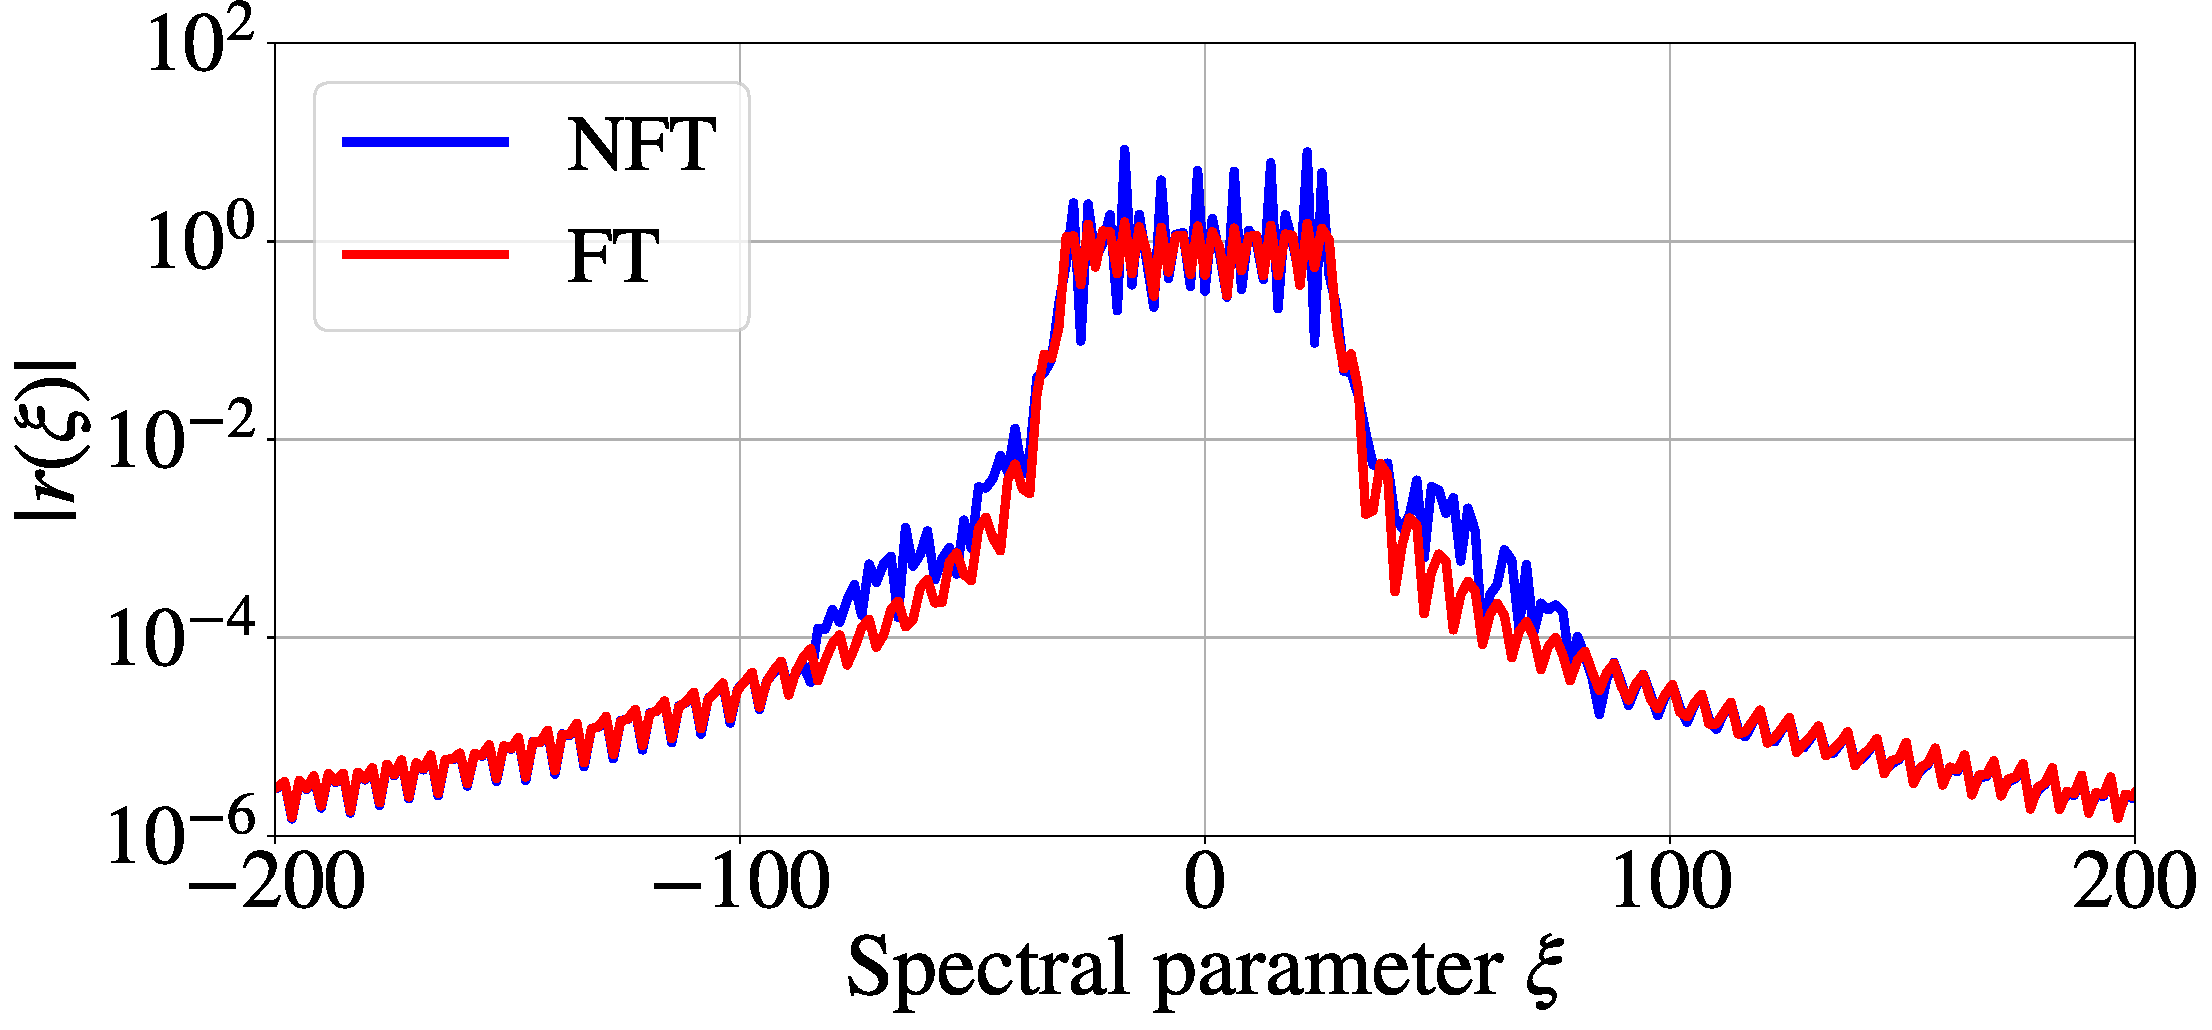
\includegraphics[width=1.\linewidth]{images/nn_nft/scirep_ft_vs_nft_actual.pdf}
  \caption{}
  \label{fig:nft_and_ft_a}
\end{minipage}%
\begin{minipage}{.49\textwidth}
  \centering
  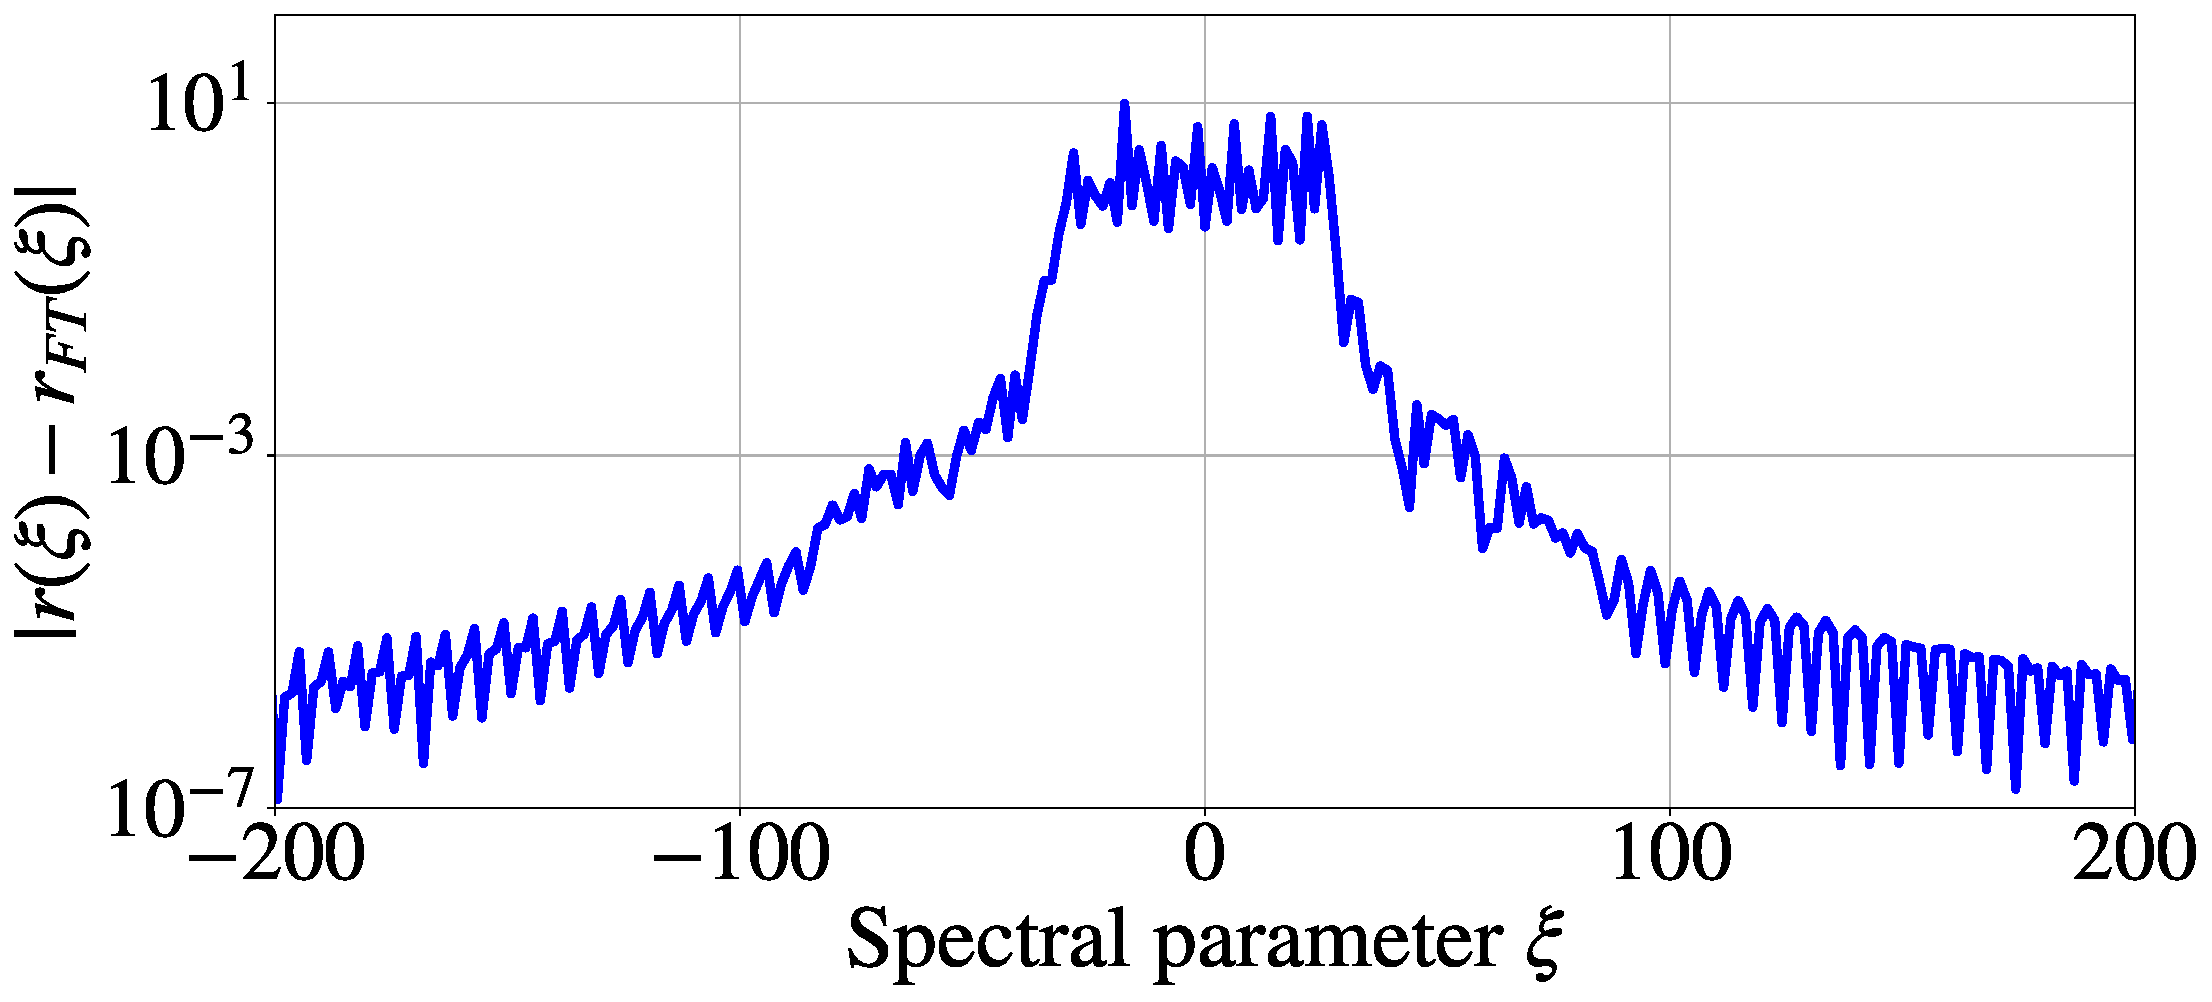
\includegraphics[width=1.\linewidth]{images/nn_nft/scirep_ft_vs_nft.pdf}
  \caption{}
  \label{fig:nft_and_ft_b}
\end{minipage}

\caption{\textbf{(a)} Example of the amplitudes of Fourier spectrum (FT) and continuous nonlinear Fourier spectrum (NFT) for one of the training signals. \textbf{(b)} Example of the absolute value of the difference between Fourier spectrum and continuous nonlinear Fourier spectrum for one of the training signal. For both graphs signal energy $E_{\text{signal}} = 39.0$ in non-dimensional units.}
\label{fig:nft_and_ft}
\end{figure}

\subsection*{Numerical NFT computation}
In our work we used the conventional forward NFT numerical method to generate training and testing data set pairs: the signal and its respective NF spectrum. %There exists a considerable amount of literature devoted to the different methods for the forward NFT operations \cite{pw18,yk14-2,vps19}.
For the computation of continuous NF spectrum associated with a given profile $q(t)$ (containing no solitons) having the form of Eq.~(\ref{eq:wdm}), we used the exponential scheme ES4 from the FNFT package\cite{FNFT2018} (non-fast realisation). It has the accuracy proportional to the fourth power of the time sample size, $\sim (\Delta t)^4$. We note that there exists the fast realisation of the NFT processing with $\sim (\Delta t)^4$ accuracy\cite{medvedev2020exponential}, which can potentially be used for efficient NFT-Net training.

\subsection*{Complexity analysis}
One of the important metrics in the development of signal processing tools is the complexity of the processing device, i.e. the number of elementary arithmetic operations that the processing unit employs to reach its goal. 
Quite often we need to analyse the interplay between the complexity and accuracy of the processing unit. Thus, here we perform the complexity analysis for the NFT-Net.

In our case, we concentrate only on the number of multiplications, since in practical implementation the computational complexity of addition operations is negligible. 
The number of real multiplications needed for the forward propagation of the model, as introduced in \cite{freire2021performance} for several types of NN layers, is also used to calculate the computational complexity of the NFT-Net in this paper. 

The overall complexity $C$ of the NFT-Net can be presented as the sum of two constituents: the complexity of densely-connected block $C_{\text{dense}}$ and the complexity of convolutional block $C_{\text{conv}}$. 
For the calculation of $C_{\text{dense}}$ the same formula as in \cite{freire2021performance} can be used, where we have $n_i$ inputs, $n_1$ neurons in the hidden layers, and $n_o$ outputs, and the complexity is defined as:
\begin{equation}
C_{\text{dense}}=  n_1*(n_{i} + n_{o}) {,}
\label{eq:c_dense}
\end{equation}

In the case of the convolution layer, we can change the equation given in \cite{freire2021performance} to measure the generalised convolutional layer complexity by taking into account the number of filters $f$ and kernel size $k$, as well as the effect of padding $p$, stride $s$, and dilation $d$. The complexity $C_{\text{conv, layer}}$ for one layer when the input shape is [$L_{in},Q_{in}$], is specified as follows:
\begin{equation}
C_{\text{conv, layer}} = k* Q_{in} * f *\left( \frac{L_{in} + 2*p -d*(k-1)-1}{s} +1\right) {,}
\label{eq:c_conv}
\end{equation}
where $Q_{in}$ denotes a number of channels, $L_{in}$ is a length of signal samples sequence.
Therefore, the total complexity of the NFT-Net used in this paper in terms of real multiplications per output sequence (1024 complex valued points) is:
\begin{equation}
C_{\text{conv}} = 2*(C_{\text{conv, 1}}+C_{\text{conv, 2}}+C_{\text{conv, 3}}+C_{\text{dense}}) {,}
\label{eq:c_total}
\end{equation}
where the factor 2 in front appears due to the use of two identical NNs to predict the real and imaginary parts of the continuous NF spectrum. Turning to our optimised architecture, to process  1024 complex signal samples, the following number of multiplication operations for the optimised architecture is required:
\begin{equation}
C_{\text{conv}} = 2*(10*2*10*1006+ 18* 10*15 * 972 + 14*15*10*320 + 3200*4096 +4096*1024) = 41598208 {.}
\label{eq:c_total_num}
\end{equation}
